\chapter*{Appendix A: Feature importance on Shapley plots}
\label{appendix:A}

In section \ref{sec:shapley}, the Shapley values were used to investigate the feature importance of the neural network. Summary plots were created to visualize the feature importance of the model, along with one waterfall plot to show how features for an individual prediction influenced the model prediction. More summary plots were created than were displayed in section \ref{sec:shapley}, those plots are displayed here.

\renewcommand{\thefigure}{A.\arabic{figure}} 
\setcounter{figure}{0} % Reset figure counter

\begin{figure}[H]
    \centering
    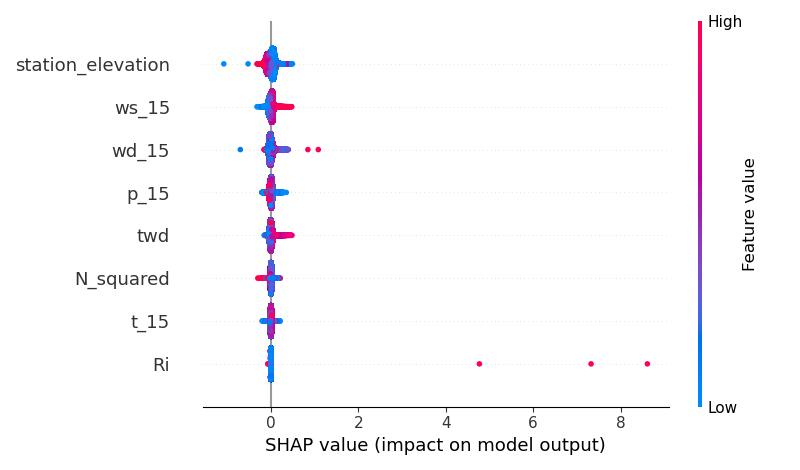
\includegraphics[scale = 0.6]{Figures/shap_plots/summary_plot_190924_full_10ms.png}
    \caption[Shapley Summary plot using entire dataset.]{Feature importance of a neural network with model architecture as described in Table \ref{table:gridSearchHyperparameters} and data as described in Table \ref{table:trainDataExample}.}
    \label{fig:ShapleySummary3}
\end{figure}

\begin{figure}[H]
    \centering
    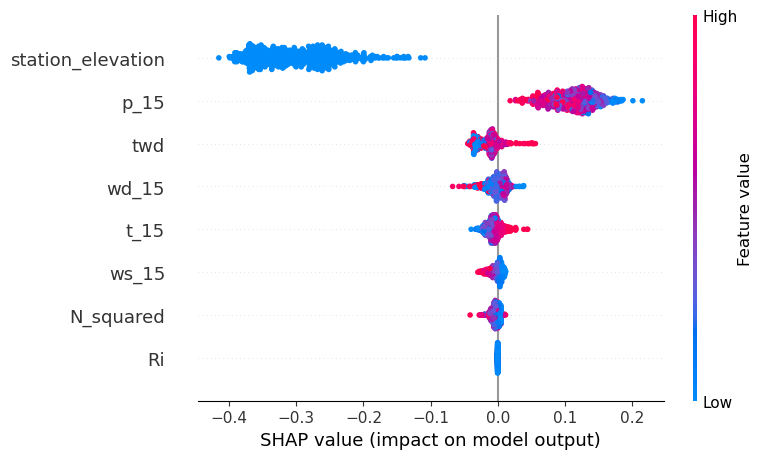
\includegraphics[scale = 0.6]{Figures/shap_plots/summary_plot_6745.png}
    \caption[Shapley Summary plot at Ásgarðsfjall.]{Feature importance of a neural network with model architecture as described in Table \ref{table:gridSearchHyperparameters} and data as described in Table \ref{table:trainDataExample}. This plot only looks at data from Ásgarðsfjall. Station elevation is influential and Richardson number has no impact.}
    \label{fig:ShapleySummaryAsgarðsfjall}
\end{figure}

\begin{figure}[H]
    \centering
    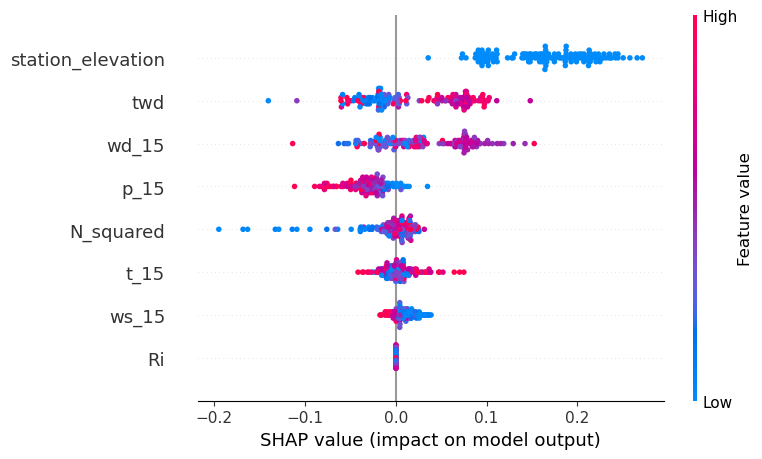
\includegraphics[scale = 0.6]{Figures/shap_plots/summary_plot_1470.png}
    \caption[Shapley Summary plot at Háahlíð.]{Feature importance of a neural network with model architecture as described in Table \ref{table:gridSearchHyperparameters} and data as described in Table \ref{table:trainDataExample}. This plot only looks at data from Háahlíð. Station elevation is influential and Richardson number has no impact.}
    \label{fig:ShapleySummaryHaahlid}
\end{figure}